\documentclass[a4paper,twoside,phd]{BYUPhys}
% The BYUPhys class is for producing theses and dissertations
% in the BYU Department of Physics and Astronomy.  You can supply
% the following optional arguments in the square brackets to
% specify the thesis type:
%
%   senior  : Produces the senior thesis preliminary pages (default)
%   honors  : Produces the honors thesis preliminary pages
%   masters : Produces the masters thesis preliminary pages
%   phd     : Produces the PhD dissertation preliminary pages
%
% The default format is appropriate for printing, with blank pages
% inserted after the preliminary pages in twoside mode so you can
% send it directly to a two-sided printer. However, for ETD
% submission the blank pages need to be removed from the final output.
% The following option does this for you:
%
%   etd     : Produces a copy with no blank pages in the preliminary section.
%             Remove this option to produce a version with blank pages inserted
%             for easy double sided printing.
%
% The rest of the class options are the same as the regular book class.
% A few to remember:
%
%   oneside : Produces single sided print layout (recommended for theses less than 50 pages)
%   twoside : Produces double sided print layout (the default if you remove oneside)
%
% The BYUPhys class provides the following macros:
%
%   \makepreliminarypages : Makes the preliminary pages
%   \clearemptydoublepage : same as \cleardoublepage but doesn't put page numbers
%                           on blank intervening pages
%   \singlespace          : switch to single spaced lines
%   \doublespace          : switch to double spaced lines
%
% --------------------------- Load Packages ---------------------------------

% The graphicx package allows the inclusion of figures.  Plain LaTeX and
% pdfLaTeX handle graphics differently. The following code checks which one
% you are compiling with, and switches the graphicx package options accordingly.
\usepackage{ifpdf}
\ifpdf
  \usepackage[pdftex]{graphicx}
\else
  \usepackage[dvips]{graphicx}
\fi

%%%%%%%%%%%%%%%%%%%%%%%%%%%%%%%%%%%%%%%%%%%%%%%%%%%%%%%%%%%%%%%%%%
% Edited : Beeshanga
%
% If you need to include any code in the text use this package
% \usepackage{listings}
% It can be used to make key words bold, add colours, etc. Refer
% to http://en.wikibooks.org/wiki/LaTeX/Packages/Listings for
% more information.
%
% For theorems, propositions, proofs and assumtions use this
% package
% \usepackage{amsthm}
% For more information refer to the following website
% http://en.wikibooks.org/wiki/LaTeX/Theorems
%
%%%%%%%%%%%%%%%%%%%%%%%%%%%%%%%%%%%%%%%%%%%%%%%%%%%%%%%%%%%%%%%%%%

% The fancyhdr package allows you to easily customize the page header.
% The settings below produce a nice, well separated header.
\usepackage{fancyhdr}
  \fancyhead{}
  \fancyhead[LO]{\slshape \rightmark}
  \fancyhead[RO,LE]{\textbf{\thepage}}
  \fancyhead[RE]{\slshape \leftmark}
  \fancyfoot{}
  \pagestyle{fancy}
  \renewcommand{\chaptermark}[1]{\markboth{\chaptername \ \thechapter. #1}{}}
  \renewcommand{\sectionmark}[1]{\markright{\thesection \ #1}}


% The cite package cleans up the way citations are handled.  For example, it
% changes the citation [1,2,3,6,7,8,9,10,11] into [1-3,6-11].  If your advisor
% wants superscript citations, use the overcite package instead of the cite package.
\usepackage{cite}

% The makeidx package makes your index for you.  To make an index entry,
% go to the place in the book that should be referenced and type
%  \index{key}
% An index entry labeled "key" (or whatever you type) will then
% be included and point to the correct page.
%\usepackage{makeidx}
%\makeindex

% The url package allows for the nice typesetting of URLs.  Since URLs are often
% long with no spaces, they mess up line wrapping.  The command \url{http://www.physics.byu.edu}
% allows LaTeX to break the url across lines at appropriate places: e.g. http://www.
% physics.byu.edu.  This is helpful if you reference web pages.
\usepackage{url}
\urlstyle{rm}

% If you have a lot of equations, you might be interested in the amstex package.
% It defines a number of environments and macros that are helpful for mathematics.
% We don't do much math in this example, so we haven't used amstex here.
\usepackage{amsmath}
\usepackage{amssymb}
\usepackage{subfigure}
\usepackage{cite}
\usepackage{amsxtra}
\usepackage{amsfonts}
\usepackage{graphicx}
\usepackage{multirow} % This is package for multi-rows in tables added on 7th July 2009 by Arif
%\usepackage{setspace}

% The caption package allows us to change the formatting of figure captions.
% The commands here change to the suggested caption format: single spaced and a bold tag
\usepackage[labelfont=bf,labelsep=colon]{caption}%[2008/04/01]
 \DeclareCaptionFormat{suggested}{\singlespace#1#2#3\par\doublespace}
 \captionsetup{format=suggested}


\usepackage{array}
\usepackage{multirow}
\usepackage{verbatim}
\usepackage{enumerate}

% Defining the symbols

% The hyperref package provides automatic linking and bookmarking for the table
% of contents, index, equation references, and figure references.  It must be
% included for the BYU Physics class to make a properly functioning electronic
% thesis.  It should be the last package loaded if possible.
%
% To include a link in your pdf use \href{URL}{Text to be displayed}.  If your
% display text is the URL, you probably should use the \url{} command discussed
% above.
%
% To add a bookmark in the pdf you can use \pdfbookmark.  You can look up its usage
% in the hyperref package documentation
\usepackage[bookmarksnumbered,pdfpagelabels=true,plainpages=false,colorlinks=true,
            linkcolor=black,citecolor=red,urlcolor=blue]{hyperref}

% ------------------------- Fill in these fields for the preliminary pages ----------------------------
%
% For Senior and honors this is the year and month that you submit the thesis
% For Masters and PhD, this is your graduation date
  \Year{2018}
  \Month{November XX,}
  \Author{Dione Morales}

% If you have a long title, split it between two lines. The \TitleBottom field defines the second line
% A two line title should be an "inverted pyramid" with the top line longer than the bottom.
  \TitleTop{Detecting health misinformation in web page text}
  \TitleBottom{using deep learning methods}
  %\TitleBottom{Line 2 of the Tile} % edited Beeshanga
 \DegreeTitle{Bachelor of Engineering
 \\ Computer Engineering Stream} % edited Beeshanga

% Your research advisor
 \Advisor{Supervisor: Associate Professor Adam Dunn}

% The department undergraduate research coordinator
%  \UgradCoord{A}

% The representative of the department who will approve your thesis (usually the chair)
%  \DepRep{B}

% Acknowledge those who helped and supported you

  \Acknowledgments{
  \vspace{-1.5cm}
    \noindent I would like to acknowledge ...

  }


% The title of the department representative
%  \DepRepTitle{Chair}
  \Statement{
    \noindent I, (insert name here), declare that this report, submitted as part of the requirement for the award of Bachelor of Engineering in the School of Engineering, Macquarie University, is entirely my own work unless otherwise referenced or acknowledged. This document has not been submitted for qualification or assessment an any academic institution.
    \vspace{0.5cm}

    \noindent     Student's Name:

    \vspace{0.25cm}

    \noindent Student's Signature:

    \vspace{0.25cm}

    \noindent     Date:
    }

% The text of your abstract
\Abstract{
\vspace{-1.5 cm}
This is where you write your abstract ...

}



% Statement of Candidate



\fussy

\begin{document}

 % Start page counting in roman numerals
 \frontmatter

 % This command makes the formal preliminary pages.
 % You can comment it out during the drafting process if you want to save paper.

 \makepreliminarypages


%\clearemptydoublepage
\doublespace
%\include{Publications/publications}

% \clearemptydoublepage
%\include{Organization/organization}

 \clearemptydoublepage
\singlespace
 % Make the table of contents.
 \tableofcontents

\clearemptydoublepage
% Make the list of figures
\listoffigures

\clearemptydoublepage
% Make the list of tables
\listoftables

\clearemptydoublepage

% Start regular page counting at page 1
\mainmatter
%
\chapter{Introduction}
\label{chap:Introduction}

  

One of the key components required to minimize the propagation of misinformation online is to have the ability of automatically evaluating and quantifying the credibility of articles. However, traditional automated methods - such as shallow learning-based techniques, still require the domain knowledge of experts to be able to develop the features required by the model. Thus, this project aims to investigate the performance of Deep Learning-based (DL) techniques in evaluating the credibility of information within domain-specific articles via the classification of set criteria that have deemed to be highly correlated with articles that have low credibility. Specifically, this project will focus on evaluating the credibility of online health articles related to vaccination due to the commonly misinformed and controversial views associated with its effects \cite{Burgess2006}. \newline


\section{Project Overview}
This section details the scope of the project and its associated outcomes outlining the various tasks that must be accomplished to successfully complete the project.

\subsection{Project Scope}
\label{sec:ProjectScope}

With the primary objective of this project being the evaluation on the effectiveness of deep learning models in determining the credibility of online health-related articles. Due to the complexity of this project, a set of activities - divided into main goals and stretch goals, have been defined to ensure that the completion of this project remains feasible in the given time frame. The completion of all activities categorized as main goals will signal the realization of the primary objective and the completion of the project. Stretch goals are activities of interest that have been identified as non-essential to the completion of the primary objective but (talk about the overarching goal that all stretch goals have in common e.g. understand the model, utilize the model etc.) and will be worked on after the completion of the project.

\subsubsection{Main Goals}
\begin{itemize}
	\item Develop a set of criteria that will be used to determine the credibility of online articles.
	\item Evaluate the performance of common ML-based methods on the classification of online vaccine-related articles, based on the criteria developed.
	\item Evaluate the performance of the proposed DL model on the classification of online vaccine-related articles, based on the criteria developed.
	\item Evaluate the effect of transfer learning methods in the performance of the proposed DL method (assuming that the chosen method doesn't rely on transfer learning)
	\item Evaluate the effectiveness of various transfer learning methods for the classification task
\end{itemize}



\subsubsection{Stretch Goals}
\begin{itemize}
	\item Utilize attention mechanisms to understand how the aforementioned DL model classifies the criteria for credibility.
\end{itemize}



\chapter{Background and Related Work}
\label{chap:LitReview}

A literature review has been conducted to develop an understanding on the research that has been done in the assessment of the credibility of information, specifically in the context of information related to health and the limitations and capabilities of shallow learning techniques and how it differs from deep learning-based methods for the task of text classification. 

\section{Assessing the Credibility of Information}

To have the capability of automating the process of evaluating the quality or credibility of online information, a definition that outlines of what is required by an article to be considered as a credible source of information must be developed. While there has been a significant amount of research that has been done on the development of tools and frameworks that aim to assess the credibility of online health information, there is currently no standardized method or benchmark that is universally used. Tools and frameworks that have been identified to be applicable in the context of this project are: DISCERN \cite{DISCERN}, HealthNewsReview \cite{HealthNewsReview} and Quality Index for health-related Media Reports (QIMR) \cite{QIMR}.

\subsection{DISCERN}
\label{sec:DISCERN}

DISCERN is a questionnaire designed to assess the reliability of a publication, it consists of 16 questions each with a Likert scale, ranging from 1 (no) to 5 (yes) and is divided into 3 sections. The first section (questions 1 - 8) investigate the reliability of the information and is comprised of questions such as "Are the aims clear?", "Is it balanced and unbiased?" and "Does it refer to areas of uncertainty?". The second section (questions 9 - 15) assesses the quality of information provided by the publication for treatment choices and is composed of questions such as "Does it describe the risks/benefits of each treatment?" and "Does it provide support for shared decision-making?". The final section (question 16) assesses the overall rating of the publication ("Based on the answers to all of the above questions, rate the overall quality of the publication as a source of information about treatment choices").

\textit{Note: Need to talk about advantages/disadvantages, limitations, relevance to this project etc.}

\subsection{HealthNewsReview}
\label{sec:HealthNewsReview}

HealthNewsReview provides a set of 10 criteria designed to act as a framework for evaluating the credibility of health-related media. The criteria is based on the various elements that all health-related media should consist of, the criteria is composed of criterion such as "Does the story compare the new approach with existing alternatives?", "Does the story use independent sources and identify conflicts of interest?" and "Does the story appear to rely solely or largely on a news release?".

\textit{Note: Need to talk about advantages/disadvantages, limitations, relevance to this project etc.}

\subsection{QIMR}
\label{sec:QIMR}

QIMR is a tool developed to monitor the quality of health research reports presented in the media. The tool considers 5 main factors that have been deemed to be correlated with the quality of research reports based on interviews with health journalists and researchers. The 5 main factors are: background information provided, sources of information used, manner in which results were analysed, context of the research and the validity of their methodology. 


\section{Prior Approaches}
\label{sec:PriorApproaches}

The task of text classification is a heavily researched topic due to its wide number of applications in various domains. Formally, text classification is defined to be the task of finding a classifier $f: D \rightarrow L$ where $D = \{d_1, d_2, \dots, d_n\} $ is a collection of documents and $L = \{l_1, l_2,\dots, l_k\}$ is the set of possible labels that a document $d$ can be classified as. 
\begin{equation}
\label{eq:TextClassification}
f: D \rightarrow L \text{ where } f(d) = l
\end{equation}
Common applications of text classification algorithms are: organization and filtering of news articles, document retrieval, opinion mining, email classification and spam filtering \cite{Aggarwal2012}. 

Traditional shallow learning-based approaches for text classification, such as Naive Bayes, Support Vector Machines (SVM) and Random Forests, require the manual extraction of features \cite{Aggarwal2012} \cite{Allahyari2017} \cite{Korde2012} \cite{Pasupa2016}. These features are typically either hand-crafted and domain specific, requiring expert-level knowledge for the task domain \cite{Pasupa2016} or are simple and general but prone to the loss of information (e.g. unable to account for context) since these features, such as term frequency-inverse document frequency (TF-IDF) scores or bag of words (BoW) models, are unable to represent and account for the sequential nature of text.

\subsection{Naive Bayes Classifier}
\label{sec:NaiveBayes}

Naive Bayes is a probabilistic classifier that functions on an assumption in how the data (i.e. the words in a document) is generated. The assumption that these Bayesian classifiers are based on is that the distribution of different words within a corpus are independent from each other. Despite this assumption clearly being wrong when considering the distribution of words within a document (due to the sequential nature of text), Naive Bayes classifiers are still able to perform well in text classification tasks such as the filtering of spam emails \cite{Sahami}.

Naive Bayes classifiers utilize Bayes' theorem, which attempts to find the probability of an event $B$ occurring given some prior condition $A$ i.e. $P(B| A)$. In the context of text classification, Naive Bayes classifiers classifies a document $d$ by calculating the probabilities that the document belongs for all labels $l_i \in L$ and then selecting the highest probability \cite{Allahyari2017}:
\begin{equation}
P(L = l_i| d) = \frac{P(l_i)P(d| l_i)}{P(d)}
\end{equation}

According to Aggarwal et al. \cite{Aggarwal2012}, there are two main types of Naive Bayes classifiers that are commonly used, they are the multivariate Bernoulli model and the multinomial model. The main discriminating factor between these two models is that the Bernoulli model does not take into account the frequency of words as it represents a document using a vector of binary features which signify the presence or absence of words, based on some vocabulary, for a given document. This is in contrast with the multinomial model, which accounts for the frequency of words as the document is represented using a BoW model. Deciding on which model to use for text classification largely depends on the size of the vocabulary as, according to McCallum et al. \cite{McCallum1998}, the multinomial models almost always outperforms the Bernoulli models if the size of the vocabulary is large ($> 1000$) or even if the size has been optimally chosen for both models.

\subsection{Support Vector Machines}
\label{sec:SVM}

SVMs are a type of supervised machine learning-based binary classifiers that are extensively used for text classification due to their capability of handling the high dimensional and sparse nature of the common techniques used to represent text documents \cite{Informatik1997}. SVMs are able to classify a document by using a hyperplane to separate the different classes into separate regions. The hyperplane used is determined by choosing the one that maximises the margin of separation (i.e. The Euclidean distance between the hyperplane and all data points in the representation space) between the two classes \cite{Aggarwal2012}.

Consider the illustration shown in figure \ref{fig:SVMExample} that presents three  two-dimensional hyperplanes, $A$, $B$ and $C$, which separates the classes 'x' and 'o'. Visually, we can determine that $A$ is the hyperplane that maximises the margin of separation, thus, $A$ will be used as a decision rule to classify any new document based on its location with respect to $A$. Mathematically, determining which hyperplane to use as the decision rule is an optimisation problem that attempts to maximise the margin represented as shown in equation \ref{eq:MaxSVM}:

\begin{equation}
	\text{maximize: } \frac{1}{2}||\frac{1}{w}||^2
	\label{eq:MaxSVM}
\end{equation}

This optimisation problem is often restructured to the minimisation of equation \ref{eq:MinSVM}:

\begin{equation}
	\text{minimize: } \frac{1}{2}||w||^2
	\label{eq:MinSVM}
\end{equation}



\begin{figure}[!h]
	\centering
	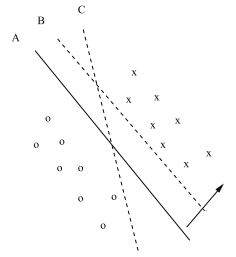
\includegraphics[totalheight=8cm]{images/svm-example.png}
	\caption{What is the Best Separating Hyperplane? \cite{Aggarwal2012}}
	\label{fig:SVMExample}
\end{figure}

\subsection{Artificial Neural Networks}
\label{sec:ANN}

A neural network consists of three kinds of layers: an input layer, hidden layer and an output layer. The differentiating factor between shallow neural networks (SNNs) and deep neural networks (DNNs) is that SNNs consist of only a single hidden layer \cite{Pasupa2016} 


\section{Deep Learning Approaches}
\label{sec:DeepLearningReview}

Deep learning models are a class of machine learning models that have the capability of automatically learning a hierarchical representation of data. These hierarchical representations are constructed through the use of artificial neural networks, the main underlying mechanism of deep learning models. Typically, large amounts of training data is required to train a model in learning the language model required to attain state of the art results, in the task of text classification for instance, the size of commonly used non-domain specific datasets range from hundreds of thousands of training examples to millions \cite{Conneau2017} \cite{Zhang} \textit{(note: look into the datasets used by state of the art approaches)}. Due to these constraints, it is not feasible to procure a dataset for the domain specific task of this project due to the aforementioned knowledge expertise and time requirements to manually label the articles required. Hence, \textit{(Talk about transfer learning/N-shot learning/domain adaptation here)} will be used to overcome this issue.

\textit{Introduce the state-of-the-art DL based approaches for text classification and try to compare it performance with state-of-the-art ML approaches} \newline
\textit{For each model, talk about the following:}
\newline
\textbf{\textit{NOTE: REMEMBER WHEN WRITING THIS SECTION TO ALWAYS CONSIDER HOW IT DIFFERS TO ML TECHNIQUES}}
\begin{itemize}
	\item \textit{How it works and the mechanisms involved}
	\item \textit{Advantages}
	\item \textit{Limitations}
\end{itemize} 

\textit{Introduce the typical architectures used for text classification e.g. RNNs, LSTMs, CNNs, GRUs?}

\subsection{Deep Learning Models}
\label{sec:DLModels}

\subsubsection{Recurrent Neural Networks}
\label{sec:RNN}

\subsubsection{Gated Recurrent Unit Networks}
\label{sec:GRU}

\subsubsection{Long Short-Term Memory Networks}
\label{sec:LSTM}

\subsubsection{Convolutional Neural Networks}
\label{sec:CNN}

\subsection{GET PROPER NAME FOR THIS SECTION}
\subsubsection{Transfer Learning}
\label{sec:TransferLearningReview}
\textit{Talk about transfer learning and how it works and how it is applicable to this project.}

\subsubsection{N-Shot Learning}
\label{sec:NShotLearningReview}
\textit{Talk about zero/few/etc-shot learning and how it works and how it is applicable to this project.}

\section{Conclusion}
\label{sec:LitReviewConclusion}
\textit{Summarize lit review and describe why DL-based approaches should be preferred over ML-based for this type of problem. Also talk about Transfer/N-Shot learning and describe which one will be feasible given the project's time constraints}

\chapter{Proposed Approach}
\label{chap:approach}

\section{Rationale}
\label{sec:ProposedRationale}
\textit{Introduce and discuss the factors that led to me choosing the proposed approach}


\section{Credibility Criteria}
\label{sect:CredibilityCriteria}
\textit{Introduce and discuss the 7 criteria that will be classified and describe how the criteria was determined}

\section{Study Data}
\label{sec:StudyData}
\textit{Talk about the data I'll be using, how we got it, its characteristics etc.}

\section{System Model}
\label{sect:chap2sysmodel}
\textit{Describe the architecture of the model}

\section{Experiments}
\label{sec:Experiments}
\textit{Describe the experiments that I'm planning to do (in such a way that they are easily reproducible)}

\section{Outcome Measures}
\label{sec:OutcomeMeasures}
\textit{Talk about the type of analyses that I'll be doing to determine the performance of my proposed model}

\chapter{Conclusions and Future Work}
\label{chap:Conclusions}


\section{Conclusions}
\label{sec:ConclusionsConclusions}

The end

\section{Future Work}
\label{FutureWork}



\clearemptydoublepage
\chapter{Abbreviations}
\label{chap:abbreviations}

\begin{tabbing}

AWGN \qquad \qquad \= Additive White Gaussian Noise\\
BC \> Broadcast Channel\\
BS \> Base Station\\
CSI \> Channel State Information\\
CSIR \> Channel State Information at Receiver\\
CSIT \> Channel State Information at Transmitter\\
dB \> Decibels\\
DPC \> Dirty Paper Coding\\
GS \> Gram-Schmidt\\
RVQ \> Random Vector Quantisation\\
SISO \> Single Input Single Output\\
SNR \> Signal to Noise Ratio\\
SINR \> Signal to Interference plus Noise Ratio\\
MISO \> Multiple Input Single Output\\
SIMO \> Single Input Multiple Output\\
MIMO \> Multiple Input Multiple Output\\
MMSE \> Minimum Mean Square Error\\
MRC \> Maximum Ratio Combining\\
QoS \> Quality of Service\\
TDD \> Time Division Duplex\\
FDD \> Frequency Division Duplex\\
ZF \> Zero-Forcing\\
ZFBF \> Zero-Forcing Beamforming\\
ZMCSCG \> Zero Mean Circularly Symmetric Complex Gaussian\\

\end{tabbing}

%\phantomsection \addcontentsline{toc}{chapter}{Index}
% \renewcommand{\baselinestretch}{1} \small \normalsize
% \printindex

\appendix
\chapter{name of appendix A}
\section{Overview}
here is the Overview of appendix A ...
\section{Name of this section}
here is the content of this section ...
\chapter{name of appendix B}
\section{Overview}
here is the Overview of appendix B ...
\section{Name of this section}
here is the content of this section ...

%\input{Bibliography/biblio3}
\bibliographystyle{IEEEtranS}
%\bibliographystyle{acm}
\bibliography{my_reference}
%\bibliography{Bibliography/biblio4}


\end{document}
